%%%%%%%%%%%%%%%%%%%%%%%%%%%%%% -*- Mode: Latex -*- %%%%%%%%%%%%%%%%%%%%%%%%%%%%
%% uhtest-appendix.tex -- 
%% Author          : Robert Brewer
%% Created On      : Fri Oct  2 16:31:12 1998
%% Last Modified By: Robert Brewer
%% Last Modified On: Mon Oct  5 14:41:05 1998
%% RCS: $Id: uhtest-appendix.tex,v 1.1 1998/10/06 02:07:03 rbrewer Exp $
%%%%%%%%%%%%%%%%%%%%%%%%%%%%%%%%%%%%%%%%%%%%%%%%%%%%%%%%%%%%%%%%%%%%%%%%%%%%%%%
%%   Copyright (C) 1998 Robert Brewer
%%%%%%%%%%%%%%%%%%%%%%%%%%%%%%%%%%%%%%%%%%%%%%%%%%%%%%%%%%%%%%%%%%%%%%%%%%%%%%%
%% 

\chapter{Other results and brief snapshot of some tables}

\begin{figure}[h]
        \caption{Inversion table depth image from the intel d435 in color}
        \centering
        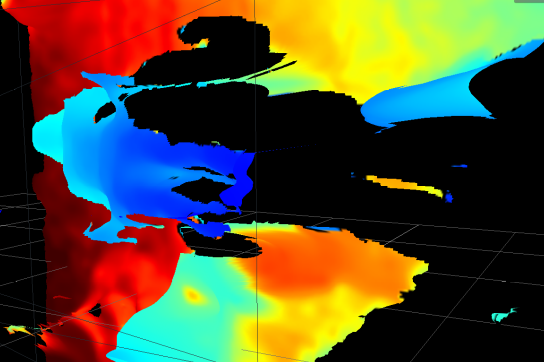
\includegraphics[width=0.7\textwidth]{images/inversion_depth.png}
\end{figure}
 

\begin{figure}[h]
        \caption{SPIN 3d reconstruction on single 2d rgb image}
        \centering
        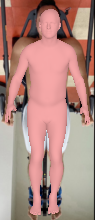
\includegraphics[width=0.3\textwidth]{images/spin.png}
\end{figure}

\begin{figure}[h]
        \caption{SMIL sample output}
        \centering
        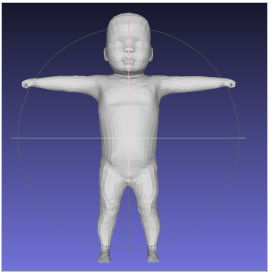
\includegraphics[width=0.4\textwidth]{images/smil.png}
\end{figure}

\begin{figure}[!htb]
        \caption{Missing data}
        \centering
        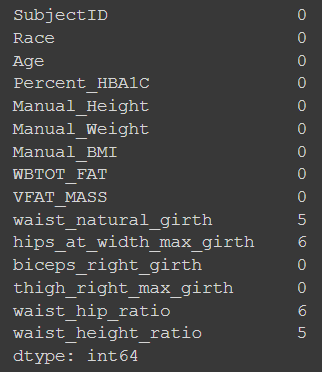
\includegraphics[]{images/missing_data.png}
\end{figure}

\begin{figure}[!htb]
        \caption{HBA1C Distribution}
        \centering
        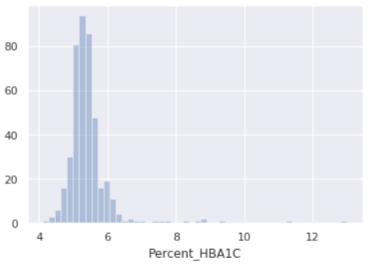
\includegraphics[width=0.5\textwidth]{images/hba1c.png}
\end{figure}

\begin{figure}[!htb]
        \caption{WBTOT FAT Distribution}
        \centering
        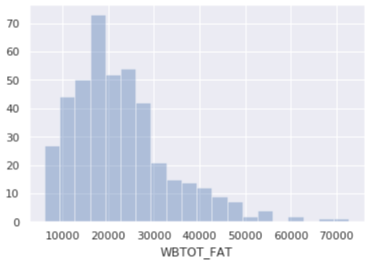
\includegraphics[width=0.5\textwidth]{images/wbtot_fat.png}
\end{figure}


\begin{figure}[!htb]
        \caption{VFAT MASS Distribution}
        \centering
        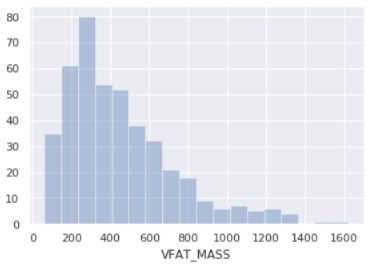
\includegraphics[width=0.5\textwidth]{images/vfat_mass.png}
\end{figure}

\begin{figure}[!htb]
        \caption{Race Ratios Distribution}
        \centering
        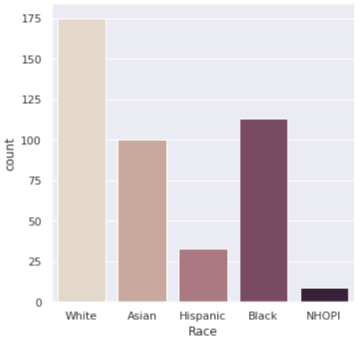
\includegraphics[width=0.5\textwidth]{images/race_ratios.png}
\end{figure}
\begin{figure}[!htb]
        \caption{Fat Mass Training Table}
        \centering
        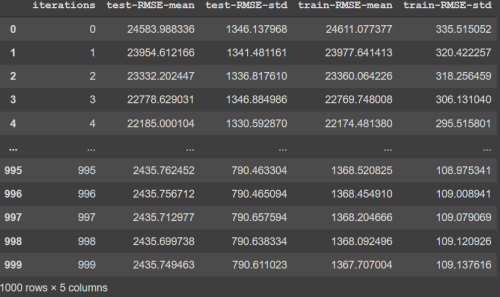
\includegraphics[width=0.7\textwidth]{images/catboost_training.png}
\end{figure}

\begin{table}[!h]
\caption{Test Table 1}
\centering
\pgfplotstabletypeset[
    col sep=comma,
    string type,
    columns/.style={column type={|l}},
    columns/.style={column type={|l}},
    columns/.style={column type={|l|}},
    columns/.style={column type={|l}},
    columns/.style={column type={|l}},
    columns/.style={column type={|l}},
    every head row/.style={before row=\hline,after row=\hline},
    every last row/.style={after row=\hline},
    ]{tables/test.csv}
\end{table}


\begin{table}[!h]
\caption{Test Table 1}
\centering
\pgfplotstabletypeset[
    col sep=comma,
    string type,
    columns/.style={column type={|l}},
    columns/.style={column type={|l}},
    columns/.style={column type={|l|}},
    columns/.style={column type={|l}},
    every head row/.style={before row=\hline,after row=\hline},
    every last row/.style={after row=\hline},
    ]{tables/test2.csv}
\end{table}

\begin{table}[!h]
\caption{Table Sensor Accuracy}
\centering
\pgfplotstabletypeset[
    col sep=comma,
    string type,
    columns/.style={column type={|l}},
    columns/.style={column type={|l}},
    columns/.style={column type={|l|}},
    columns/.style={column type={|l}}, 
    columns/.style={column type={|l}},
    columns/.style={column type={|l|}},
    columns/.style={column type={|l}},
    every head row/.style={before row=\hline,after row=\hline},
    every last row/.style={after row=\hline},
    ]{tables/accuracy.csv}
\end{table}
% Setup siunitx:
\sisetup{
  round-mode          = places, % Rounds numbers
  round-precision     = 2, % to 2 places
}
\begin{table}[!h]
\caption{Table Sensor Temporal Noise}
\centering
\pgfplotstabletypeset[
    col sep=comma,
    string type,
    columns/.style={column type={|l}},
    columns/.style={column type={|l}},
    columns/.style={column type={|l|}},
    columns/.style={column type={|l}}, 
    columns/.style={column type={|l}},
    columns/.style={column type={|l|}},
    columns/.style={column type={|l}},
    every head row/.style={before row=\hline,after row=\hline},
    every last row/.style={after row=\hline},
    ]{tables/temporal-noise.csv}
\end{table}

\begin{table}[!h]
\caption{Table Fill Rate}
\centering
\pgfplotstabletypeset[
    col sep=comma,
    string type,
    columns/.style={column type={|l}},
    columns/.style={column type={|l}},
    columns/.style={column type={|l|}},
    columns/.style={column type={|l}}, 
    columns/.style={column type={|l}},
    columns/.style={column type={|l|}},
    columns/.style={column type={|l}},
    every head row/.style={before row=\hline,after row=\hline},
    every last row/.style={after row=\hline},
    ]{tables/fill-rate.csv}
\end{table}

\begin{figure}[!htb]
        \caption{Connected Components Best Mesh 1}
        \centering
        \includegraphics[width=0.5\textwidth]{images/cc_best_mesh_1.png}
\end{figure}
\begin{figure}[!htb]
        \caption{Connected Components Best Mesh 2}
        \centering
        \includegraphics[width=0.5\textwidth]{images/cc_best_mesh_2.png}
\end{figure}
\begin{figure}[!htb]
        \caption{Connected Components Best Mesh 3}
        \centering
        \includegraphics[width=0.5\textwidth]{images/cc_best_mesh_3.png}
\end{figure}

\begin{figure}[!htb]
        \caption{Connected Components Worst  Mesh 3}
        \centering
        \includegraphics[width=0.5\textwidth]{images/cc_worst_mesh_4.png}
\end{figure}

\begin{figure}[!htb]
        \caption{Connected Components Worst  Mesh 2}
        \centering
        \includegraphics[width=0.5\textwidth]{images/cc_worst_mesh_5.png}
\end{figure}

\begin{figure}[!htb]
        \caption{Connected Components Worst  Mesh 3}
        \centering
        \includegraphics[width=0.5\textwidth]{images/cc_worst_mesh_6.png}
\end{figure}

\begin{figure}[!htb]
        \caption{Closest mesh by euclidean distance}
        \centering
        \includegraphics[width=0.5\textwidth]{images/euclidean_ideal.png}
\end{figure}

\begin{figure}[!htb]
        \caption{A fully labeled mesh, all 300,000 vertices colored by closest landmark}
        \centering
        \includegraphics[width=0.5\textwidth]{images/full_labeled_mesh.png}
\end{figure}

\begin{figure}[!htb]
        \caption{A subsampled labeled mesh by color}
        \centering
        \includegraphics[width=0.5\textwidth]{images/labeled_mesh.png}
\end{figure}

\begin{figure}[!htb]
        \caption{Ideal mesh reposed through Meshcapade}
        \centering
        \includegraphics[width=0.5\textwidth]{images/reposed_mesh.png}
\end{figure}

\begin{figure}[!htb]
        \caption{Turntable speed}
        \centering
        \includegraphics[width=0.5\textwidth]{images/turntable_speed.png}
\end{figure}


